\section{Per-head Paired Intervals}
\label{app:intervals}
Table~\ref{tab:intervals} reports nominal 95\% paired test-example intervals for the primary Early-5 base-feature estimator. Gains and bounds are percentage points. The TTA reference in each interval uses the same view count as that head, which can differ from the globally validation-selected uniform-TTA policy in Table~\ref{tab:accuracy}. No interval here compares independently sampled datasets or directly tests Early-5 against the static regressor.
\begin{table}[!ht]
\centering\scriptsize
\caption{Primary estimator: saved validation-selected policies and conditional paired intervals.}
\label{tab:intervals}
\begin{tabular}{llrrrrr}
\toprule
Run & Head seed & Views & $T$ & Gain & CI vs base & CI vs same-view TTA \\
\midrule
C100, base 42 & 42 & 5 & 0.05 & +1.10 & [+0.57, +1.65] & [+0.61, +1.49] \\
C100, base 42 & 43 & 5 & 0.02 & +1.10 & [+0.54, +1.63] & [+0.56, +1.53] \\
C100, base 42 & 44 & 5 & 0.05 & +0.68 & [+0.15, +1.24] & [+0.20, +1.07] \\
C100, base 43 & 42 & 5 & 0.05 & +1.20 & [+0.70, +1.73] & [+0.86, +1.68] \\
C100, base 43 & 43 & 5 & 0.02 & +0.97 & [+0.42, +1.53] & [+0.58, +1.51] \\
C100, base 43 & 44 & 5 & 0.05 & +0.98 & [+0.48, +1.52] & [+0.63, +1.50] \\
C10 Worse, base 42 & 42 & 10 & 0.02 & +1.31 & [+0.88, +1.76] & [+0.50, +1.22] \\
C10 Worse, base 42 & 43 & 10 & 0.02 & +1.34 & [+0.90, +1.79] & [+0.52, +1.26] \\
C10 Worse, base 42 & 44 & 10 & 0.02 & +1.32 & [+0.87, +1.79] & [+0.51, +1.24] \\
\bottomrule
\end{tabular}

\end{table}

\clearpage
\section{Calibration and Error Ranking}
\label{app:calibration}
AUROC uses original-view scores and fixed original-view base-error labels. ECE, NLL, and Brier use the final probabilities of each method's selected policy. Therefore the ranking and calibration columns refer to explicitly different evaluation objects. Figure~\ref{fig:calibration_changes} shows changes relative to the corresponding base. All values for learned heads are arithmetic means over three head seeds; no seed is chosen by test performance.
\begin{table}[!ht]
\centering\scriptsize
\caption{Error AUROC and final-probability calibration. Lower ECE, NLL, and Brier are better.}
\label{tab:calibration}
\begin{tabular}{llrrrr}
\toprule
Run & Method & AUROC $\uparrow$ & ECE $\downarrow$ & NLL $\downarrow$ & Brier $\downarrow$ \\
\midrule
C100, base 42 & Base & 0.8124 & 0.1200 & 1.1253 & 0.4362 \\
C100, base 42 & Uniform TTA & 0.8124 & 0.1610 & 1.1670 & 0.4500 \\
C100, base 42 & Entropy weighting & 0.7647 & 0.1610 & 1.1670 & 0.4500 \\
C100, base 42 & Static & 0.8045 & 0.1554 & 1.1587 & 0.4465 \\
C100, base 42 & History-50 & 0.7112 & 0.1459 & 1.1570 & 0.4434 \\
C100, base 42 & Early-5 & 0.8307 & 0.1291 & 1.1404 & 0.4348 \\
C100, base 43 & Base & 0.8222 & 0.0963 & 1.1313 & 0.4358 \\
C100, base 43 & Uniform TTA & 0.8222 & 0.1436 & 1.1814 & 0.4503 \\
C100, base 43 & Entropy weighting & 0.7799 & 0.1436 & 1.1814 & 0.4503 \\
C100, base 43 & Static & 0.7984 & 0.1433 & 1.1810 & 0.4501 \\
C100, base 43 & History-50 & 0.6953 & 0.1335 & 1.1707 & 0.4434 \\
C100, base 43 & Early-5 & 0.8326 & 0.1098 & 1.1541 & 0.4363 \\
C100, base 44 & Base & 0.8281 & 0.0888 & 1.1082 & 0.4286 \\
C100, base 44 & Uniform TTA & 0.8281 & 0.0888 & 1.1082 & 0.4286 \\
C100, base 44 & Entropy weighting & 0.7874 & 0.0888 & 1.1082 & 0.4286 \\
C100, base 44 & Static & 0.8059 & 0.0888 & 1.1082 & 0.4286 \\
C100, base 44 & History-50 & 0.7097 & 0.1124 & 1.1476 & 0.4402 \\
C100, base 44 & Early-5 & 0.8325 & 0.0989 & 1.1375 & 0.4338 \\
C10 Worse, base 42 & Base & 0.8764 & 0.2847 & 0.6203 & 0.2677 \\
C10 Worse, base 42 & Uniform TTA & 0.8764 & 0.3155 & 0.6532 & 0.2841 \\
C10 Worse, base 42 & Entropy weighting & 0.8048 & 0.2464 & 0.5601 & 0.2373 \\
C10 Worse, base 42 & Static & 0.8853 & 0.3033 & 0.6382 & 0.2757 \\
C10 Worse, base 42 & History-50 & 0.7689 & 0.2888 & 0.6260 & 0.2687 \\
C10 Worse, base 42 & Early-5 & 0.9064 & 0.2756 & 0.5903 & 0.2481 \\
C10 Worse, base 43 & Base & 0.8758 & 0.2518 & 0.5591 & 0.2420 \\
C10 Worse, base 43 & Uniform TTA & 0.8758 & 0.2893 & 0.5903 & 0.2559 \\
C10 Worse, base 43 & Entropy weighting & 0.8312 & 0.2877 & 0.5877 & 0.2546 \\
C10 Worse, base 43 & Static & 0.8792 & 0.2886 & 0.5890 & 0.2552 \\
C10 Worse, base 43 & History-50 & 0.7398 & 0.2673 & 0.5659 & 0.2422 \\
C10 Worse, base 43 & Early-5 & 0.8976 & 0.2542 & 0.5359 & 0.2254 \\
\bottomrule
\end{tabular}

\end{table}

\begin{figure}[!ht]
\centering
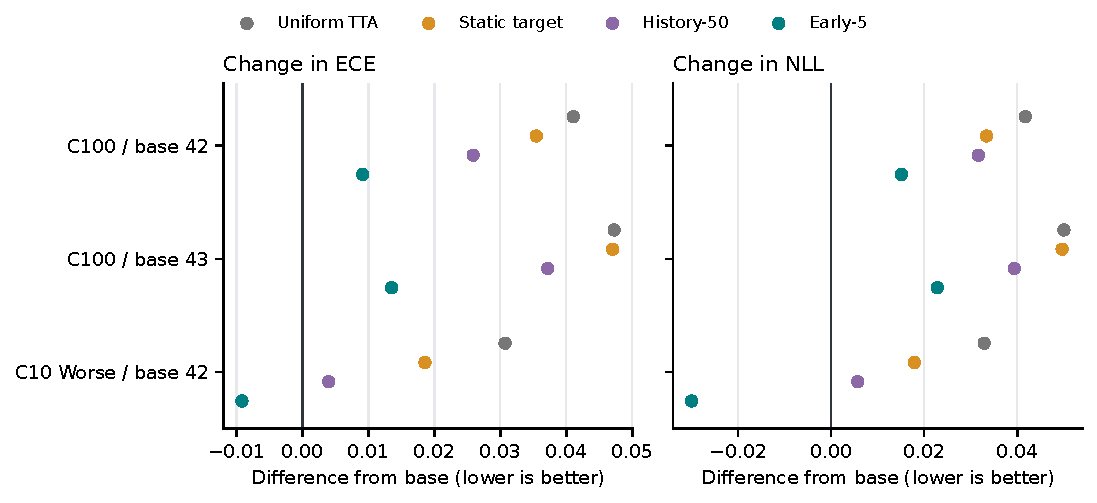
\includegraphics[width=\linewidth]{figures/calibration_changes.pdf}
\caption{Change in final-probability calibration relative to the corresponding base. Points average learned heads where applicable. Positive values mean worse ECE or NLL. These are point estimates, not confidence intervals; methods use their own validation-selected policies.}
\label{fig:calibration_changes}
\end{figure}

\section{Reconstruction of the Regression Targets}
Table~\ref{tab:reconstruction} measures prediction of the corresponding scalar target on the 6,750 diagnostic IDs excluded from PCA fitting, head fitting, and head checkpoint selection. These images were seen by the base during its training. The static target is reconstructed more accurately than Early-5 despite its lower downstream accuracy; target reconstruction and usefulness for inference are distinct properties. Values are averaged over three head seeds, separately for each base.
\begin{table}[!ht]
\centering\small
\caption{Diagnostic-held-out target reconstruction using base features. $R^2$ is relative to each target's own variance; it is not error-detection AUROC.}
\label{tab:reconstruction}
\begin{tabular}{llrr}
\toprule
Run & Target & MSE & $R^2$ \\
\midrule
C100, base 42 & Early-5 & 0.0519 & 0.754 \\
C100, base 42 & Static & 0.0493 & 0.838 \\
C100, base 42 & History-50 & 0.1085 & 0.524 \\
C100, base 43 & Early-5 & 0.0511 & 0.753 \\
C100, base 43 & Static & 0.0542 & 0.828 \\
C100, base 43 & History-50 & 0.1066 & 0.539 \\
C100, base 44 & Early-5 & 0.0538 & 0.743 \\
C100, base 44 & Static & 0.0589 & 0.816 \\
C100, base 44 & History-50 & 0.1087 & 0.547 \\
C10 Worse, base 42 & Early-5 & 0.0187 & 0.917 \\
C10 Worse, base 42 & Static & 0.0051 & 0.980 \\
C10 Worse, base 42 & History-50 & 0.0748 & 0.810 \\
C10 Worse, base 43 & Early-5 & 0.0182 & 0.918 \\
C10 Worse, base 43 & Static & 0.0055 & 0.982 \\
C10 Worse, base 43 & History-50 & 0.0759 & 0.808 \\
\bottomrule
\end{tabular}

\end{table}

\section{Reproducibility Details}
The regressor's scalar output is internally broadcast to 50 entries for compatibility with the existing trajectory-prediction interface. MSE over this repeated target is mathematically the same scalar regression objective; it does not train 50 independent outputs. Stable sample IDs link trajectories, features, annotations, and views. PCA is fitted separately for each encoder using only meta-training features. The ResNet18 condition retains all 512 dimensions without whitening; the base-feature condition reduces 2048 dimensions to 512.

The observed-label static target uses an unaugmented forward pass at the selected checkpoint, while temporal targets use training-time augmentations and changing weights. The matched comparison holds the head and decision procedure fixed, but target construction differs in both temporal information and measurement conditions. A fixed-checkpoint target averaged over the same augmentation process would further separate those contributions.

